\documentclass[11pt]{article}
\usepackage{ragged2e}
\usepackage[utf8]{inputenc}
\usepackage[catalan]{babel}
\usepackage{hyperref}
\usepackage{graphicx}
\usepackage{array}
\usepackage{afterpage}
\graphicspath{ {Images/} }

\begin{document}
\begin{titlepage}

\newcommand{\HRule}{\rule{\linewidth}{0.5mm}} % Defines a new command for the horizontal lines, change thickness here

\center % Center everything on the page
 
%----------------------------------------------------------------------------------------
%	HEADING SECTIONS
%----------------------------------------------------------------------------------------

\textsc{\LARGE Universitat de Lleida}\\[1.5cm] % Name of your university/college

\includegraphics{Images/logoUDL.jpg}\\[1cm] % Include a department/university logo - this will require the graphicx package
\textsc{\Large Grau en Enginyeria Informàtica}\\[0.5cm] % Major heading such as course name
\textsc{\large Xarxes}\\[0.5cm] % Minor heading such as course title

%----------------------------------------------------------------------------------------
%	TITLE SECTION
%----------------------------------------------------------------------------------------

\HRule \\[0.4cm]
{ \huge \bfseries Pràctica 1, Programació d’aplicacions de xarxa}\\[0.4cm] % Title of your document
\HRule \\[1.5cm]
 
%----------------------------------------------------------------------------------------
%	AUTHOR SECTION
%----------------------------------------------------------------------------------------

\begin{minipage}{0.4\textwidth}
\begin{flushleft} \large
\emph{Autor:}\\
Jordi Ricard Onrubia Palacios % Your name
\end{flushleft}
\end{minipage}
~
\begin{minipage}{0.4\textwidth}
\begin{flushright} \large
\emph{Professor:} \\
Enric Guitart % Supervisor's Name
\end{flushright}
\end{minipage}\\[4cm]

%----------------------------------------------------------------------------------------
%	DATE SECTION
%----------------------------------------------------------------------------------------
{\large \today}\\[3cm] % Date, change the \today to a set date if you want to be precise
\vfill % Fill the rest of the page with whitespace
\end{titlepage}

%%%%%%%%%%%%%%%%%%%%%%%%%%%%%%%%%
%%%%%%%%%%%%ABSTRACT%%%%%%%%%%%%%
%%%%%%%%%%%%%%%%%%%%%%%%%%%%%%%%%
\newpage
\section*{Resum}
En el següent document es troba la informació necessaria per a comprende el funcionament del client i el servidor proposats per la pràctica. Per a la seva explicació es dan ús de diagrames de estats on es mostra el funcionament dels protocols emprats. Per a mostrar la implmentació del client i el servidor s'explique l'estructuració juntament amb diagrames de execució, on es mostren les funcions utilitzades i com s'executen entre elles. 
\justify
\thispagestyle{empty}
%%%%%%%%%%%%%%%%%%%%%%%%%%%%%%%%%
%%%%%%%%%%%%INDEX%%%%%%%%%%%%%%%%
%%%%%%%%%%%%%%%%%%%%%%%%%%%%%%%%%
\newpage
\thispagestyle{empty}
\tableofcontents
%%%%%%%%%%%%%%%%%%%%%%%%%%%%%%%%%
%%%%%%%%%%%%COS%%%%%%%%%%%%%%%%%%
%%%%%%%%%%%%%%%%%%%%%%%%%%%%%%%%%
\newpage
\clearpage
\pagenumbering{arabic}
\section{Protocol UDP}
Some text
\begin{figure}[h]
    \centering
    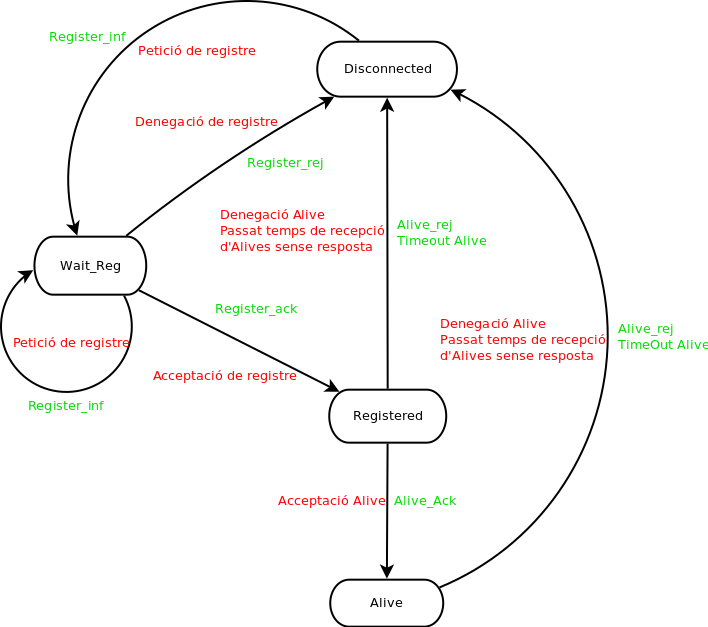
\includegraphics[width=0.8\textwidth]{UDP_diagram.png}
    \caption{Protocol UDP}
    \label{fig:ProtcolUDP}
\end{figure}

\section{Protocol TCP}
\newpage
\section{Client}
\justify
Programat en: Python versió 2.7.10.\\\\
El client està dividit en 2 fases diferents:
\subsection*{Primera fase: Registre}
Per a la primera fase el client al iniciar-se fa un intent de registre al servidor mitjançant el protocol UDP, un cop finalitzant l'intent de registre passem a la següent fase.
\\\\
Com es pot observar en la figura \ref{fig:Client} la comunicació entre les funcions que intervenen en la primera fase sòn aquelles numerades del 1 al 18.
\subsection*{Segona fase: Manteniment de comunicació i espera de comandes per teclat}
En la segona fase intervenen processos el primer encarregat de mantenir la comunicació i el segon encarregat de rebre comandes per teclat, per tal de que aquests processos facin les seves funcions previament caldrà comprovar que el registre a estat realitzat correctament.\\\\
La comunicació entre les funcions que intervenen en la comprovació correcta del registre sòn aquelles numerades del 19 al 24.\\\\
La comunicació entre les funcions que intervene en la espera de comandes per teclat és aquella numerada amb el 25 on es crea la bifurcació entre els processos i aquelles numerades del 26 al 40.\\\\
La comunicació entre les funcions que intervenen en el manteniment de la comunicació és aquella numerada amb el 25 on es crea la bifurcació entre els processos i aquelles numerades del 41 al 45.
\afterpage{\clearpage}
\begin{figure}[h]
    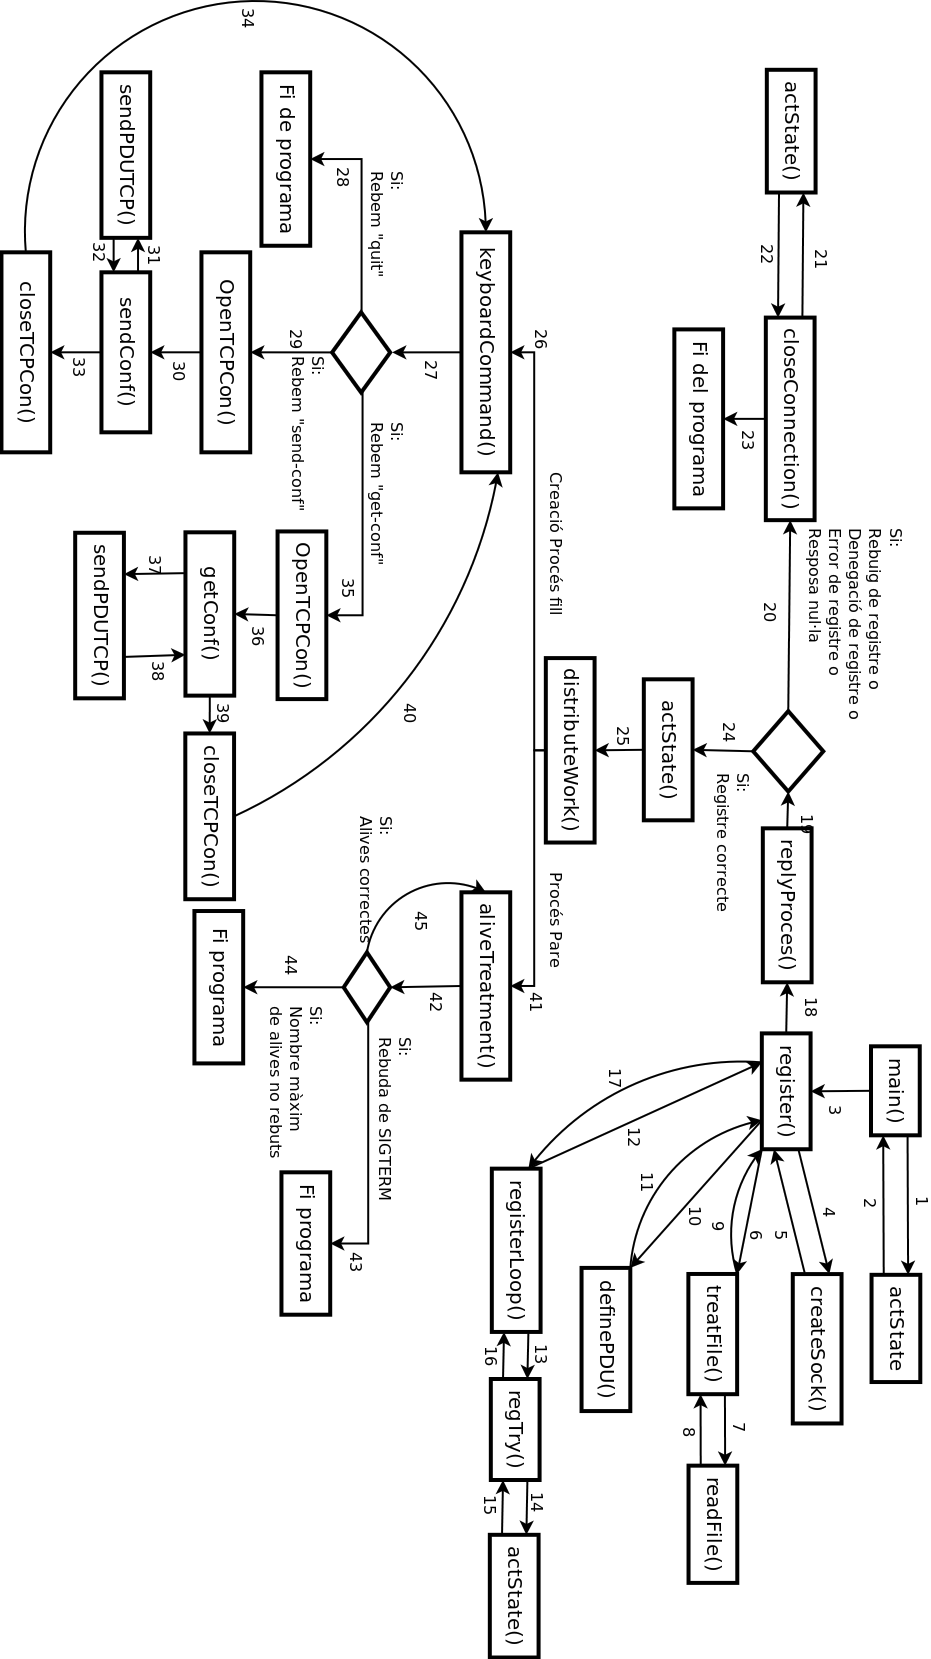
\includegraphics[width=0.8\textwidth]{Client.png}
    \caption{Client}
    \label{fig:Client}
\end{figure}
\newpage
\section{Servidor}
Compilat en: Linux versió 4.2.0 gcc versió 5.2.1.\\
Comanda utilitzada: gcc -ansi -pedantic -Wall.
%%%%%%%%%%%%%%%%%%%%%%%%%%%%%%%%%
%%%%%%%%%%%%ANEXE%%%%%%%%%%%%%%%%
%%%%%%%%%%%%%%%%%%%%%%%%%%%%%%%%%
\newpage
\section{Anexe}
	\subsection{Execució}
		\subsubsection*{Client:}
Execució:
\begin{itemize}
\item Executar el fitxer client.py de la següent manera: python client.py
\item És important que el fitxer cons.py estigui en el mateix arxiu que client.py ja que aquest conté totes les constants que han de ser utiltizades en la execució del client.
\end{itemize} 
		\subsubsection*{Servidor:}
Compilació:
\begin{itemize}
\item Executar el fitxer Makefile inclós de la següent manera: ./Makefile.
\item Si el fitxer Makefile no pot ser executat per falta de permisos executar la comanda: chmod +x Makefile. 
\item És important que el fitxer server.c estigui en el mateix arxiu que el Makefile.
\end{itemize}
Execució:
\begin{itemize}
\item Executar el fitxer server generat per Makefile desprès de la seva execució de la següent manera: ./server
\item Si el fitxer server no pot ser executat per falta de permisos executar la comanda: chmod +x server.
\end{itemize}
	\subsection{Problemes i solucions trobats en el desenvolupament}
		\subsubsection*{Client}
\begin{enumerate}
\item Bloqueig del programa per part del recvfrom, recvfrom és una funció què s'encarrega de rebre el missatge rebut pel socket, la solució aplicada va ser posar el timeout a 0 fent-la així no bloquejant.
\item Senyal SIGTERM ignorada, la solució aplicada va ser enviarl-la continuament amb un bucle infinit.
\item Llançament de excepcions per part de Python a l'hora de detectar per teclar un ctrl-c, ls solució aplicada va ser tractar la lectura del teclat amb un try except ignorant les interrupcions de teclat.
\end{enumerate}
		\subsection*{Servidor}
\begin{enumerate}
\item Problema d'accedir i actualitzar les dades dels clients des d'altres processos. La solució ha estat fer un mmap utilitzant la llibreria sys/man.h.
\item Si els dos primers ''ALIVES'' la temporització no arriba a agafar el tercer ''ALIVE'' en cas de què fos enviat, ja que aquest arriba just en el moment en què el servidor a desconnectat al client. La solució ha estat aplicar un temporitzador per tal de què el servidor només comprovi els estats dels clients cada segon en lloc de continuament, a més a més, es permet que el temps en què haguera d'arribar ''l'ALIVE'' sigui més gran que l'especificat, exactament 1 segon més.
\end{enumerate}
	\subsection{Llistat de figures}
\listoffigures{}
\newpage
\section{Bibliografia}
Importar constants d'un altre fitxer en Python 2.\\
\url{http://zetcode.com/lang/python/packages/}\\
Structs en Python 2.\\
\url{https://docs.python.org/2/library/struct.html}\\
UDP sockets en Python 2.\\
\url{https://wiki.python.org/moin/UdpCommunication}\\
Funcions de la llibreria Time de Python 2.\\	
\url{https://docs.python.org/2/library/time.html}\\
TCP sockets en Python 2.\\
\url{https://wiki.python.org/moin/TcpCommunication}\\
Signals en Python 2.\\	
\url{https://docs.python.org/2/library/signal.html}\\
UDP sockets en C.\\
\url{https://www.cs.rutgers.edu/~pxk/417/notes/sockets/udp.html}\\
TCP sockets en C\\
\url{http://www.linuxhowtos.org/C_C++/socket.htm}	\\
Compartir memória en C.\\
\url{http://man7.org/linux/man-pages/man2/mmap.2.html}\\
Funcions de la llibreria Time de C.\\
\url{http://www.cplusplus.com/reference/ctime/}\\
\end{document}